\section{Introduction}
Deep convolutional neural networks are currently the leading technique for image classification.
Convolutional layers capture patterns with spatial locality, while deep topologies capture the compositional nature of images.
The problem of \emph{video} classification introduces a new, temporal dimension not leveraged by typical 2D CNNs. For instance, a video of a human subject may contain temporal concepts such as gestures or gait that cannot be extracted from a single frame. This prompts the question:
 how can we best capture the additional information contained within this temporal dimension?   

There are indeed methods of preprocessing temporal information into a single 2-dimensional input~\cite{brox}, but a more attractive research goal is to develop a neural network that can discover temporal relationships on its own.
There are multiple recent approaches towards this goal, but as of yet no consensus on which is superior.

The difficulties in training neural networks on video input include the following: memory requirements (particularly if 3D convolutions are used), fewer public data sets, size of the data sets (for instance, the Sports-1M data set is $\approx 4TB$ large), and a lack of consensus on which structural approaches are most effective.

In just the last two years, a variety of techniques have been investigated, including 3-dimensional convolutional neural networks (3D-CNN) and Long Short-Term Memory (LSTM). Additional techniques have been incorporated within these strategies, such as slow-fusion, optical-flow, and retraining of pre-trained ImageNet networks.

The purpose of this project is to examine and compare these approaches, while comparing to an additional, novel technique that we introduce that uses a second CNN layer to extract temporal information from sequentially-generated ImageNet vectors. 

We make the following contributions:
\begin{enumerate}
\item Implement and analyze a 2D-CNN $\to$ LSTM architecture for video classification.
\item Introduce and analyze a novel 2D-CNN $\to$ 2D-CNN architecture (``TCNN'') for video classification. 
\item Investigate the effect of replacing the first CNN with state-of-the-art ImageNet architectures.
\end{enumerate}

\section{Background}
While neural networks were once limited to small, toy applications, 
their power has increased dramatically due to the explosion in data 
due to social media and the rise in computational power due to GPUs. 
The ImageNet data set~\cite{imagenet}, containing millions of labeled images, has become a standard image-classification benchmark, with improvements each year from architectural tweaks~\cite{alexnet,vggnet,nin,resnet}.

With video input we must process a collection of frames. Incorporating the changes between these frames then becomes the new research problem. \emph{Slow fusion} is one of the first approaches taken, which uses multiple windows of frames. Each window is used as an input to a separate CNN, which is then combined with the results of the other convolutions into a later CNN~\cite{cnnvid}. This allows for short-term and longer-term temporal information to be taken into account. 

If a video is taken to be a projection of 3D objects onto a 2D plane, the point-wise velocities of the projected objects corresponds to a 2D motion field. Optical flow is an approximation of this field produced through analyzing consecutive frames~\cite{brox}, and is a popular feature in the video classification approaches we have examined. Unfortunately, computing optical flow accurately is numerically intensive. 

A more natural idea is the use of Recurrent Neural Networks (RNNs), which are neural networks that allow self-loops, and thus unfold over a time dimension. A crucial innovation for RNNs is Long Short-Term Memory(LSTM)~\cite{LSTM}, which uses memory cells to store, modify,
and access an internal state. While a standard RNN is limited to storing parameters related to a fixed window of time, LSTMs can discover long-range
temporal relationships. The internal mechanisms of LSTM allow this discovery to selectively store and forget the necessary information, allowing a limited number of parameters to represent a global view of the data. 

Another elegant idea is to simply extend the 2-dimensional CNN to 3 dimensions, where the third dimension is temporal. While applying a 2D convolution kernel to a 2D or 3D volume will produce a 2D volume, applying a 3D convolution kernel to a 3D volume produces another 3D volume, as illustrated in~\RefFigure{fig:3dconv}. This allows the model to incorporate the temporal dimension as an intrinsic aspect at all levels of the network, as opposed to flattening it out early on. 
\begin{figure}[ht]
  \centering
  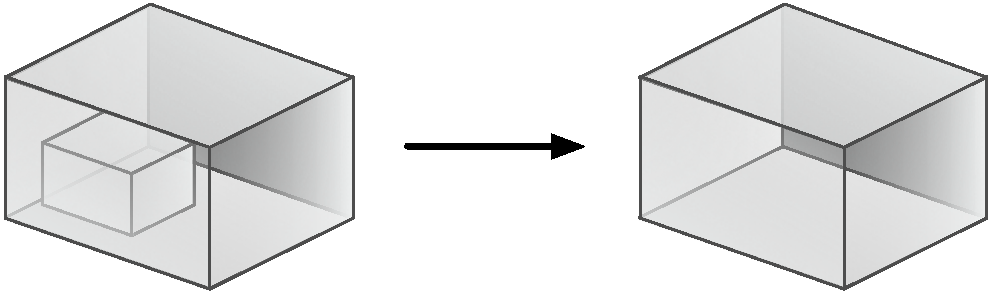
\includegraphics[width=0.7\linewidth]{figs/3dconv}
  \caption{Applying a 3D convolution produces another 3D volume.}
  \label{fig:3dconv}
\end{figure}

\subsection{Related Work}
%What has been done in similar fields/problems? What are the limitations of current approaches?
%Recurrent long-term convolutional models are most frequently used in speech and language applications, but it is possible to apply them to visual time-series data. 
The \emph{slow fusion} approach, mentioned earlier, has been applied to video input by Karpathy, et al~\cite{cnnvid}. This approach, applied to a simple CNN, shows only a modest improvement over CNN single-frame learning.

Using an LSTM has also been implemented; Donahue, et al. apply a 2D-CNN to each frame of the video, followed by an RNN with LSTM~\cite{ltrcn}. 
Ng, et al. demonstrate that instead of training on `short snippets' (such as in~\cite{cnnvid,stf}), an LSTM approach allows us to train on entire videos efficiently~\cite{snip}, and achieve state-of-the-art performance on several data sets. 

Hu, et al \cite{cnnMNLS} demonstrate in natural language processing that instead of using an RNN (or LSTM), a CNN can also be used as temporal encoder to extract sequences of information from sentences. This is an innovation that we will apply later with our novel `TCNN' network. 
% Tran, et al. demonstrated that using 3D-CNNs instead of 2D can achieve state-of-the-art results on several data sets~\cite{stf}.

Tran, et al. demonstrate that by using a 3D Convolutional Neural Network, it is possible to build a classifier on a moving window of frames using 3D convolutions to extract useful local movement information, and it can achieve state-of-the-art results on several data sets~\cite{stf}. However, 3D-CNNs introduce a massive memory blowup that may make training infeasible on GPUs.

Many of these papers incorporate additional features such as optical flow~\cite{brox} and improved dense trajectory, both of which involve optimization techniques applied to subsets of frames. 

\section{Approach and Techniques}
%What is your proposed approach to solving the problem? How does it compare to existing approaches?
%Note: It's OK for these projects to be similar to existing approaches, although if you want to publish the results they will have to have some novelty.
We have decided on combining two possible approaches, which address
the third, temporal dimension in different ways: Convolutional Neural
Networks (3D-CNNs or CNN as temporal encoder)~\cite{stf,cnnvid,cnnMNLS} and Long
Short-Term Memory /Recurrent Neural Networks (Regular or Multi-dimensional LSTM)~\cite{ltrcn}. 

\subsection{Baseline}
Our baseline model is constructed from the pretrained ImageNet CNN. For the pretrained CNN model we tried both 12-layer NIN and 101-layer Resnet. We fine-tuned the pretrained CNN model (with 2048D feature output) with an extra hidden layer with 512 features and an output layer to map the hidden layer to 101 output. After that, we then applied this fine-tuned CNN model to features of each of the input frames. A simple averaging process is used on the set of output vectors to produce a predicted class for the entire video -- essentially implementing a voting procedure. This is shown in~\reffig{fig:cnn}. This method treats each single frame individually and doesn't assume any temporal dependency between them. 
\begin{figure}
  \centering
  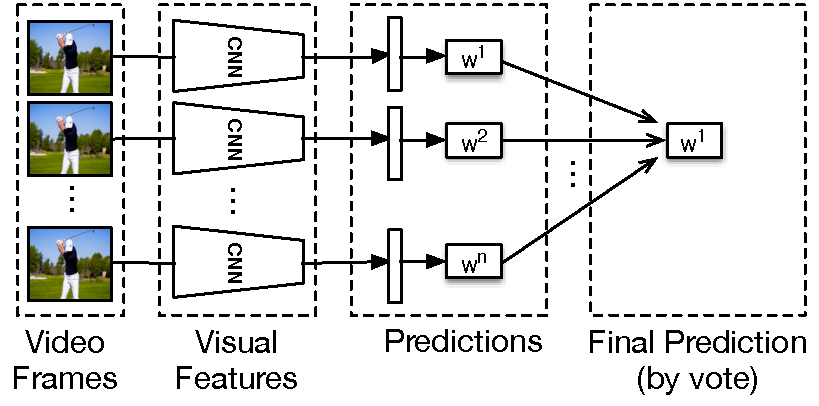
\includegraphics[width=1.0\linewidth]{figs/cnn}
  \caption{Static CNN Network}
  \label{fig:cnn}
\end{figure}

% \subsection{3D CNN}
% % 3D-CNNs
% Using a 3D Convolutional Neural Network, it is possible to build a classifier on a moving window
% of frames using 3D convolutions to extract useful local movement information. However, 3D-CNNs introduce a massive memory blowup that may make training infeasible on GPUs.
% To address this, we would like to use the slow-fusion model~\cite{cnnvid} instead of 3D kernels. In addition, we also plan to apply 3D kernels to one or two layers to check the improvement if we don't meet the memory problem.


% LSTM
\subsection{RNN with LSTM}
An RNN with LSTM approach is able to build the classifier with long term memory using a much larger number of frames at once. 
Also for applications involve temporal informations, it is natural to apply RNN. In this approach, we basically follow the work from ~\cite{ltrcn} and implement the RNN with LSTM which is designed for taking image features as input. The CNN is this LRCN model serves as a translator which converts the raw image pixel into meaningful representations for machines. On the other hand, the RNN serves as the decision module to decide whether if this video belongs to a certain types of classes. The RNN will learn the genetic representation of feature vectors across all frames for all vidoes. It learns to identify the correlation between feature vectors and the importance of some elements for different activities. 
This approach is illustrated in~\reffig{fig:lcrn}.
\begin{figure}
  \centering
  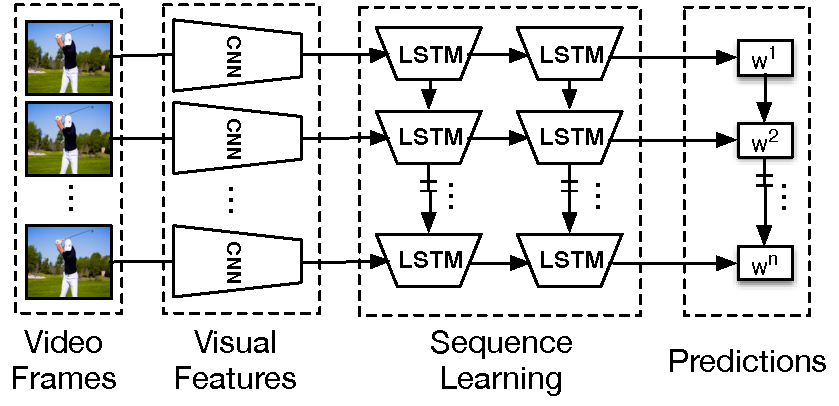
\includegraphics[width=1.0\linewidth]{figs/lcrn}
  \caption{LRCN Network}
  \label{fig:lcrn}
\end{figure}

% Furthermore, the current LSTM model is built on the fully-connected
% layer, which does not conserve spatial information. We would like to examine the 
% effectiveness of adding the LSTM network at earlier layers.
% If we apply LSTM directly after the convolution layer,
% the input to LSTM model is actually multi-dimensional tensor. To address
% this challenge, we would like to apply the multi-dimensional LSTM
% \cite{byeon2015scene} to efficiently take advantage of the spatial
% information following an early convolution layer. 

\subsection{Temporal CNN}
% CNN + CNN (1D convolution) ==> Min-Hung Chen
In addition to using the LSTM model for the temporal encoder, convolutional architecture(CNN) has also been applied to model sentences using a pre-trained embedding of words ~\cite{cnnSC,cnnMNLS}. We explore this idea and to see how it performs on high level applications such as video classification. First, similar to what we did for LCRN model described above, a pre-trained CNN architecture can be applied as a spatial encoder to each frame to extract features. 
Secondly, we concatenated feature vectors into a feature matrix and apply CNN on this particular temporal feature matrix. The CNN with 1D or 2D convolutional kernels will be applied to the temporal feature matrix separately to verify their influences. For 1D CNN, we take 1D convolution and 1D max-pooling on a sliding window of the concatenated feature vectors along with the temporal direction. For 2D CNN, we apply 2D convolution and 2D max-pooling directly on the a sliding window of the feature matrix from the spatial encoder. This approach is illustrated in~\reffig{fig:tnn}.
The idea behind this temporal CNN is that, CNN is known for extracting the stationary information in the image (or feature matrix). Using this characteristic of CNN and applying directly on feature matrices which contain temporal information can be interpreted as: we are exploring some of the distinct feature elements that consistently show up for most of the feature vectors in different time steps, and with different hierarchical layers from CNN to explore the correlation of these elements. All these distinct features and their correlations in each of the video will determine which type of activities for this video. 

\begin{figure}
  \centering
  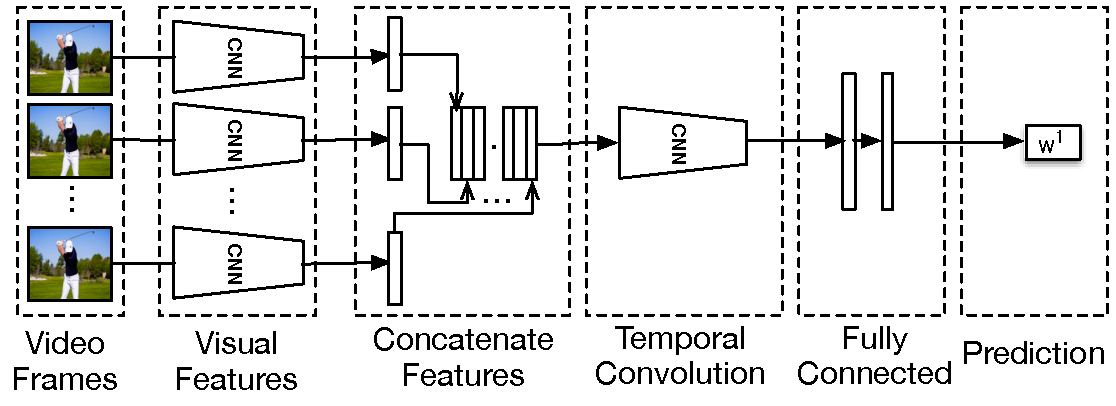
\includegraphics[width=1.0\linewidth]{figs/tnn}
  \caption{Temporal CNN Network}
  \label{fig:tnn}
\end{figure}

\section{Experiments}
\subsection{Data Set}
We target the well-established data set \emph{UCF-101}~\cite{ucf101}, which contains 13320 videos from 101 action categories. For early training purposes we used a small subset of 10 sports, and then applied to the entire dataset. The ultimate goal, not yet completed, is to apply our framework to Sports-1M~\cite{cnnvid} dataset, which contains around 1 million YouTube videos belonging to 487 categories. Some categories example of UCF101 are shown in~\RefFigure{fig:ucf101}.

\begin{figure}
  \centering
  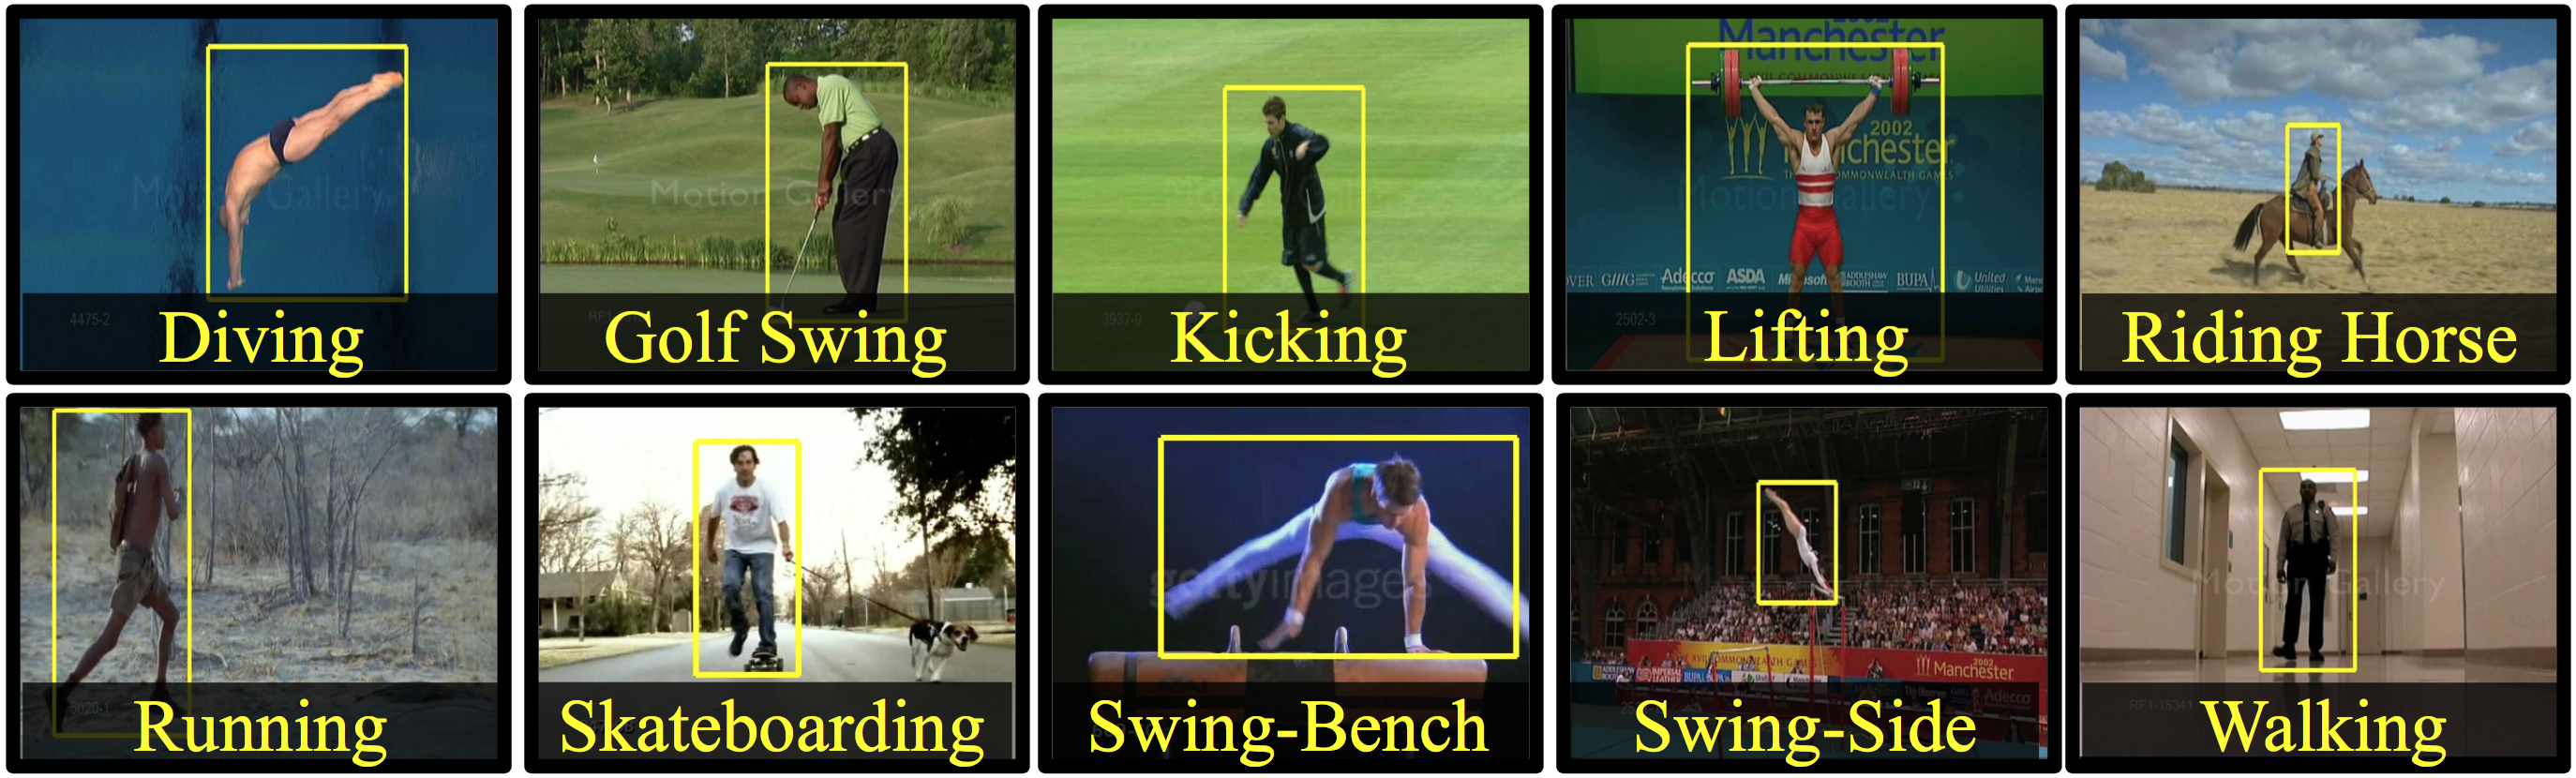
\includegraphics[width=1.0\linewidth]{figs/ucf101.png}
  \caption{10 Exmaples of UCF101}
  \label{fig:ucf101}
\end{figure}



\subsection{Experimental Methodology}
%What specific experiments are you planning on conducting? How are they testing the specific problem you want to solve?
We performed our experiments on personal computers with Intel i7-6700K, 32 GB RAM, and Nvidia GTX 980 GPU. At the begining of the experiments when we moved on to UCF-101 dataset, we randomly divided the entire dataset into 5 folds and achieve over $94\%$ accuracy at early stage using NIN model as our feature extractor. 
To compute our testing error in a way that is comparable with other publications, we used the first given training/testing data splits from the UCF-101 data set~\cite{ucf101}. Within our three models (Baseline CNN, LSTM, TCNN) we used a wide variety of pre-trained ImageNet models as the first CNN layer. These models are labeled in our experimental results. 

% The following is a set of proposed experiments, some of which we have started:
% \begin{itemize}
% \item Move 2D-LSTM within convolution layers to see if this better incorporates spatial information.
% \item Incorporate slow fusion within a 2D-CNN to see if this input approach yields higher accuracy.
% \item Replace a 2D-CNN-LSTM network with a Shallow ResNet-LSTM network (with or without slow fusion)-- to see if ResNet provides significant gains over the AlexNet used by existing studies.
% \item Study if slow-fusion \emph{combined} with optical-flow input provides significantly better results than either approach on its own.
% \item Using CNN + LSTM as base line compare with the performance from CNN + 1D-CNN/2D-CNN.

% \end{itemize}

\subsection{Results}
In Figures~\ref{fig:democorrect}--\ref{fig:demo} we show examples of the video output that our model produces. The first label is the result from the RNN model, and the second label from the T-CNN model. The first figure shows a correct classification by both models, the second incorrect classification by both models. In the third figure, the RNN model makes a misprediction while the T-CNN model is correct.  

\textcolor{red}{We should be able to elaborate and discuss more for the example images here. We need more images...} 


\begin{figure}
  \centering
  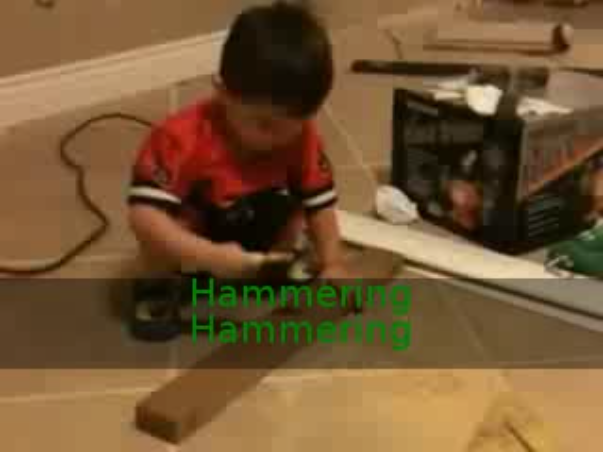
\includegraphics[width=0.8\linewidth]{figs/democorrect}
  \caption{Example of video correctly classified by both models.}
  \label{fig:democorrect}
\end{figure}


\begin{figure}
  \centering
  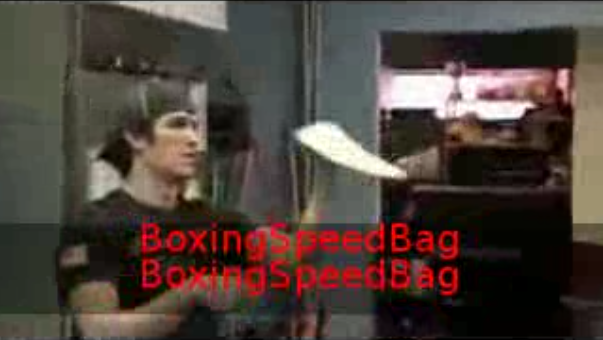
\includegraphics[width=0.8\linewidth]{figs/demoincorrect}
  \caption{Example of video incorrectly classified by both models (the correct class is PizzaThrowing)}
  \label{fig:demoincorrect}
\end{figure}

\begin{figure}
  \centering
  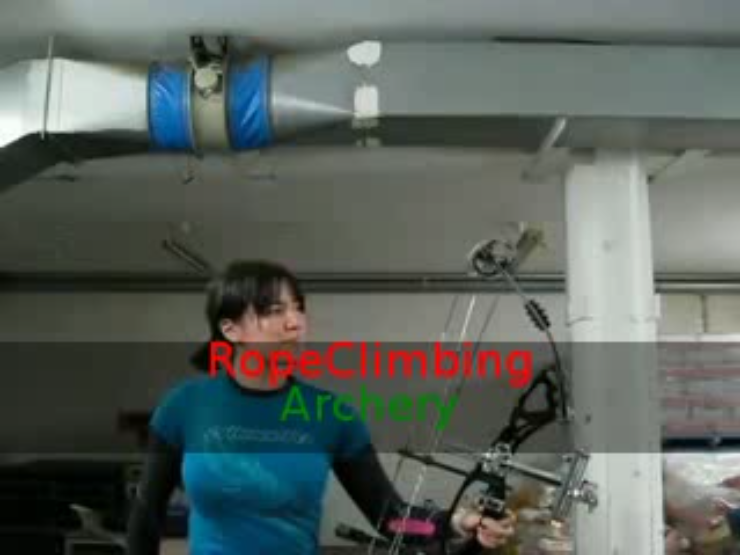
\includegraphics[width=0.8\linewidth]{figs/demo}
  \caption{Example of video correctly classified by LSTM, incorrectly classified by TCNN. }
  \label{fig:demo}
\end{figure}


In~\RefFigure{fig:cnntest} we see the training and testing error for the baseline model. The ResNet model performs over 10\% better than the NIN model, which is about the difference we'd expect for static image classification. 
\begin{figure}
  \centering
  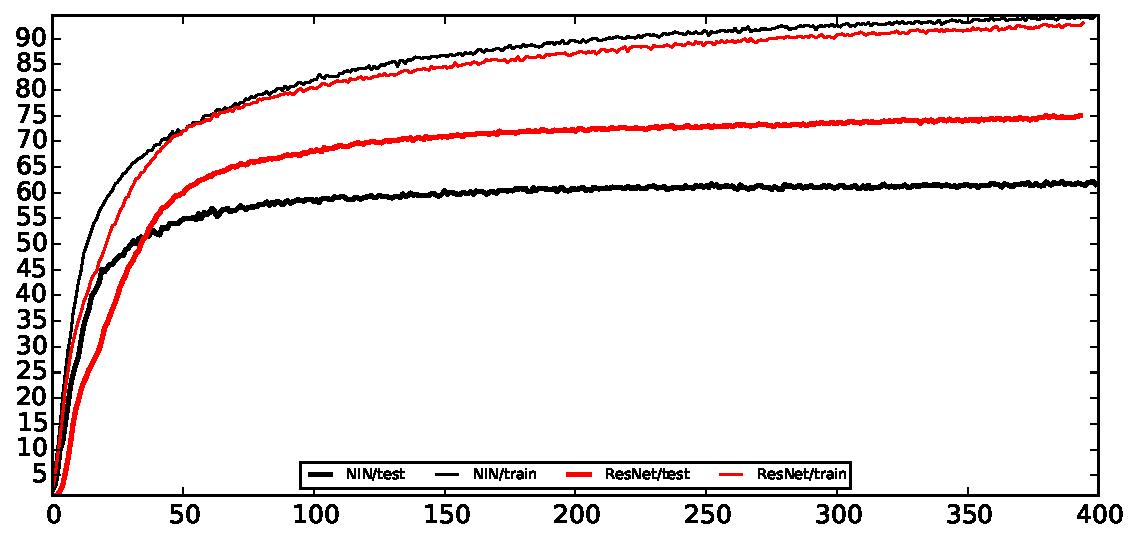
\includegraphics[width=1.0\linewidth]{figs/CNNout}
  \caption{CNN Training and Test Error}
  \label{fig:cnntest}
\end{figure}

We present the training and testing results for the LSTM model in~\RefFigure{fig:lstmtest}. The models vary in which ImageNet model is used for the first layer. Again, we see that ResNet performs the strongest, and we also expect that the deeper ResNet networks perform incrementally better than shallower ones. During the training for RNN with LSTM, we also compare the performance if we use GRU, yet the results are very similar. No significant difference observed during this experiment. 

We also tried various learning rate and settle for $5e-4$ when using adam as optimizer. Using adam as optimizer gives faster and the best convergence. It requires relatively smaller learning rate compared with using SGD. 

The number of the hidden layers are also important to learn the generic representation of the videos. Generally, hidden layer using the half of the dimension of the feature vector from CNN produce the best performance. Stacked of LSTM doesn't always help, but will not make the testing accuracy worse. 
\begin{figure}
  \centering
  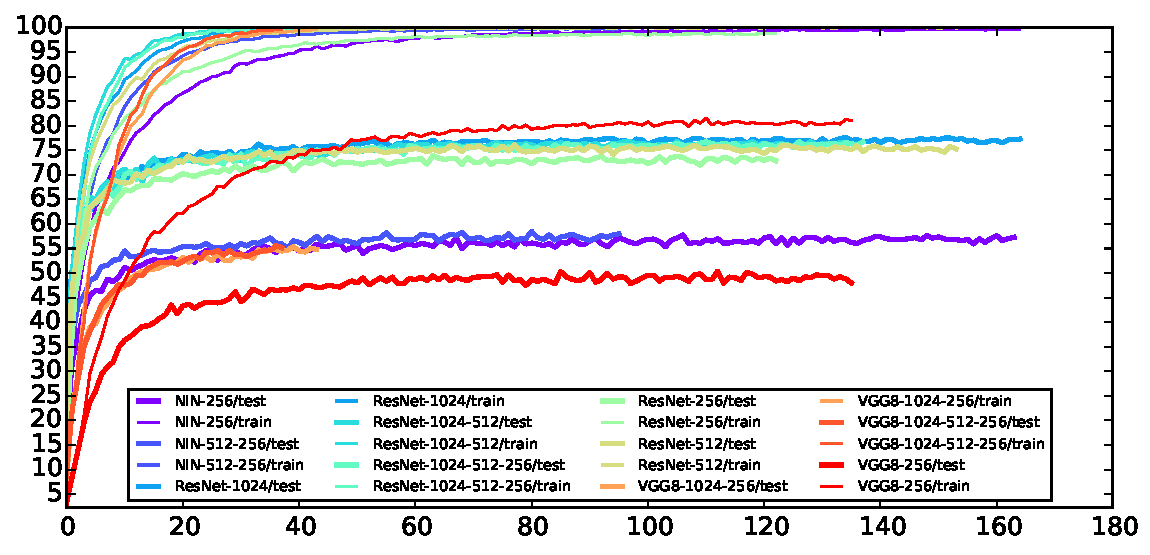
\includegraphics[width=1.0\linewidth]{figs/RNNout}
  \caption{LSTM Training and Test Error}
  \label{fig:lstmtest}
\end{figure}

Before we tested our TCNN model on the first training/testing data split from the UCF-101 dataset, we started from tuning parameters of a 2-layer architecture using NIN features and tested it on the random 5-fold validation scheme to see the influence of each parameter. We found that the parameters of layers should be gradually increased, which means having the convolution kernel size of the second layer greater than the first layer provide better performance. In addition, increasing the difference of the convolution kernel size of two layers results in better accuracy. This means we should keep the size of first layer small and the size of second layer large. We also found the pooling size affects the performance to some extent, so we should have small pooling size since larger pooling size means losing more information. According to the experiments on parameters, our first model is a 2-layer architecture with 3 hidden states (32,64, and 256), along with 2 convolution layers (kernel size 3 and 11) and 2 max-pooling layers (kernel size 4 and 2). The first pooling size is 4 due to the memory issue. (GTX 980 only has 4 GB memory)

After obtaining our primary architecture, we tested it on the first data split of UCF-101 and also tried to modified the architecture. The training and testing results for our novel TCNN method are presented in~\RefFigure{fig:tnntest}. We did the following tests: First, for the 2-layer architecture, besides the 32-64-256 model, we also tried to adopt the idea of 
LeNet~\cite{lenet} and tried a 20-50-250 model because we only train and test on 48-frame videos, which have similar size as MNIST images. However, from ~\RefFigure{fig:tnntest} we can see that the 32-64-256 model is still better by 1\%. Secondly, in addition to the 2-layer architecture, We also tried one convolution layer because the input size along the temporal direction is not large, and we don't really need deep network. The results show that the 1-layer model is slightly better than the 2-layer model using NIN features (by 2\%). Thirdly, we compared 1D kernels and 2D kernels, and found that 2D kernels don't provide better performance. It's reasonable because there is no correlation between different elements within one feature vector of a frame. Therefore, convolution along spatial direction doesn't help explore information. Finally, we changed the model of spatial CNN encoders to ResNet-101, and this improved the performance a lot. However, in this case, the 2-layer model outperformed the 1-layer model by around 3\%. 

The best results appear in the 2-layer architecture with ResNet-101 features, and the optimizer is SGD with the learning rate $1.5e-4$. The current best accuracy is 75.1\%

\begin{figure}
  \centering
  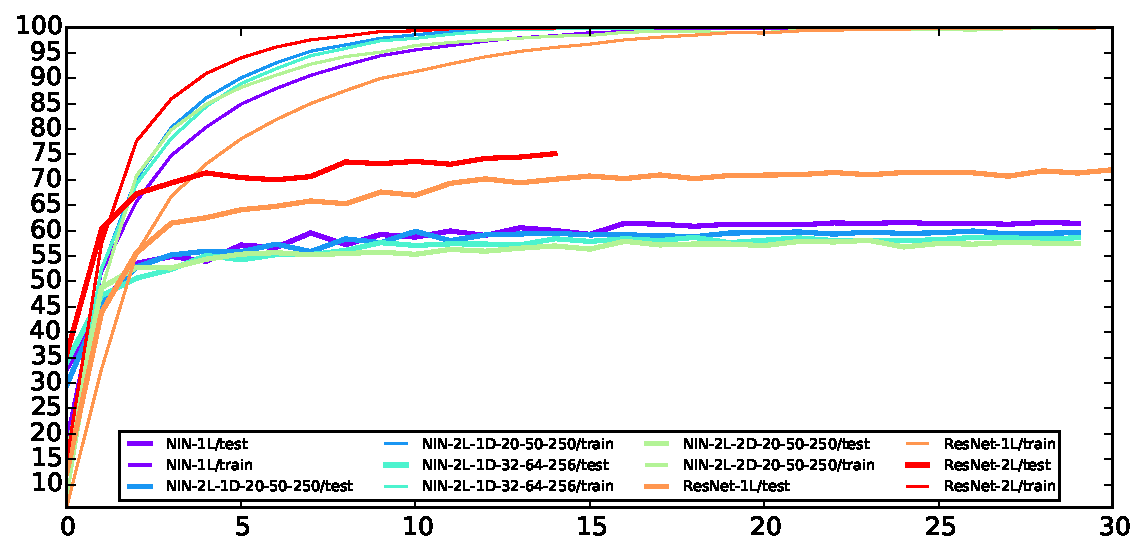
\includegraphics[width=1.0\linewidth]{figs/TCNNout}
  \caption{Temporal CNN Training and Test Error}
  \label{fig:tnntest}
\end{figure}

\begin{table}[h!]
 \caption{Best test results for a given train-test split of UCF101~\cite{ucf101}}\label{tab:cmp}
\centering
 \begin{tabular}{||l l||}
 \hline
 \textit{Our Results} & \\ \hline
 CNN (ResNet) & 74.97\% \\
 CNN-LSTM (ResNet) & \textbf{79.39\%} \\
 TCNN (Res-2L) & 75.1\% \\ \hline
 \textit{Published Results} & \\ \hline
 LRCN~\cite{byeon2015scene} & 71.12\% \\
 C3D~\cite{stf} & \textbf{85.2\%}\footnotemark \\
 SlowFusion~\cite{cnnvid} & 65.4\%\\ [0.5ex]
 \hline
 \end{tabular}
\end{table}
\footnotetext{Uses a specially trained ImageNet}

We compared our results with other state-of-the-art methods as shown in Table~\ref{tab:cmp}. It shows that our methods outperform others except the C3D~\cite{stf} method. However, C3D uses 3D kernels for convolution and pooling, and this will cause severe memory issues. In addition, they train their network using 2 huge datasets: I380K (Facebook's private big dataset) and Sports-1M. This means that they have much more training data than we do. Therefore, by using the same training data, our results will get closer to C3D and even outperform it.

\section{Conclusion and Future Work}
Perhaps the most noticeable result is that the quality of the first convolutional layer is very important. We were able to see excellent improvements in quality just by using ResNet in place of earlier ImageNet models. While we used a standard pretrained ImageNet model for this layer, we might expect improvements by further training this first layer on relevant video classes. 

Data volume is very important. We had 10000 videos in our data set, but C3D was able to train on one million videos, as well as a proprietary Facebook data set. In earlier work, Karpathy, et al. demonstrated that additional training on the Sports-1M data-set raised their testing accuracy on UCF-101 from 41.3\% to 65.4\%~\cite{cnnvid}, so we would expect large gains from training on a larger data set as well. We will explore this direction in the future work. 

The temporal CNN was not as effective as the LSTM model, and in fact only performed incrementally better than the raw CNN model. Performing convolutions across feature vectors is tricky-- while one dimension corresponds to temporal changes of the feature vectors, the other dimension (between elements of a given feature vector) does not have a clear interpretation. In addition, tuning the size of the convolution kernel (or alternatively, tuning the granularity with which frames are chosen) is a large experiment which we did not have time and the hardware to perform. As the layer of temporal CNN grows, the requirement of memory will increase drastically. However, as we move along after the project poster, we achieved over 77\% accuracy for Temporal CNN by training on CPU, and we expect to perform at least similar to the RNN after we experiment temporal CNN with more layers. 


Ultimately, we have demonstrated excellent performance of close to 80\% classification accuracy on a video set of 101 classes. We have confirmed the efficacy of previous proposed methods while experimenting with the novel TCNN model. By using the newest ImageNet models we were able to greatly exceed previous published results. 

Future work would include training on larger data sets such as Sports-1M and fine-tuning the TCNN model. Another possible future work would be using a \emph{multi-dimensional} LSTM. The current LSTM model is built on the fully-connected layer, which does not conserve spatial information. We would like to examine the effectiveness of adding the LSTM network at earlier layers. If we apply LSTM directly after the convolution layer, the input to LSTM model is actually multi-dimensional tensor. To address this challenge, we would like to apply the multi-dimensional LSTM
\cite{byeon2015scene} to efficiently take advantage of the spatial information following an early convolution layer. 

Our codes are written with Torch7 library and are available at~\url{http://github.com/cjbattagl/deeplearningproj}.
